\section{The performance-complexity trade-off problem}

The main aim of this work is to explore the performance-complexity characteristics in the context of graph learning, as described for example by \cite{prochazka_downstream_2022}. Consider an undirected graph \( G \) with nodes \( V \left( G \right) \) and edges \( E \left( G \right) \). The result of the graph coarsening part of the algorithm is a sequence of graphs \( G_0, G_1, G_2, \dots, G_L \) where \( G_0 = G \) and \( L \in \mathfield{N} \) is a hyper-parameter of the method.
Given a model \( M \) that operates on graphs, a performance metric \( P \left( G, M \right) \) and a complexity metric \( C \left( G, M \right) \), the sequence \( G_0, G_1, \dots, G_L \) can be plotted in the performance-complexity space, where the original graph \( G_0 \) usually provides the best performance and incurs the most complexity and subsequent coarsened graphs improve complexity and hurt performance. -- see Figure \ref{fig:performance-complexity} for an illustration.

\begin{figure}
  \centering
  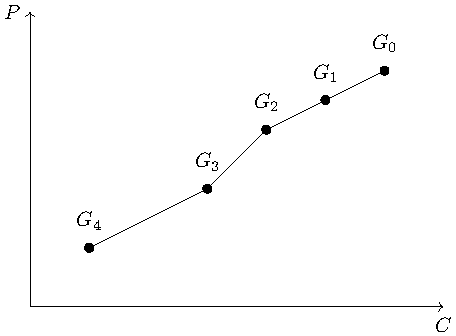
\includegraphics[width=0.45\textwidth]{images/performance-complexity/performance-complexity.pdf}
  \caption{An example of a performance-complexity curve for a sequence of graphs.}
  \label{fig:performance-complexity}
\end{figure}

This performance-complexity characteristics allows for a choice of an optimal \textbf{working point} for the model M - i.e., the choice of the optimal coarsening level \( G_i \). The choice of the working point is subjective and dependent on the particular use-case, downstream task and the environment in which the model is to be deployed. In general, however, two distinct uses of the characteristics emerge:
\begin{itemize}
  \item Finding the most performant model for a given complexity budget. That is, for a given maximum allowable complexity \( C_\mathrm{max} \), a graph \( G_i \) is to be found that maximizes \( P \left( G_i, M \right) \) while maintaining \( C \left( G_i, M \right) \leq C_\mathrm{max} \).
  \item Finding the least complex model satisfying a performance target. That is, for a given minimum acceptable performance \( P_\mathrm{min} \), a graph \( G_i \) is to be found that minimizes \( C \left( G_i, M \right) \) while maintaining \( P \left( G_i, M \right) \geq P_\mathrm{min} \).
\end{itemize}

